\documentclass[border=10pt]{standalone}

\usepackage{tikz}
\usepackage{tikzsymbols}
\usetikzlibrary{calc,patterns,shapes.geometric}

\def\centerarc[#1](#2)(#3:#4:#5){\draw[#1] ($(#2)+({#5*cos(#3)},{#5*sin(#3)})$) arc (#3:#4:#5);}

\begin{document}
	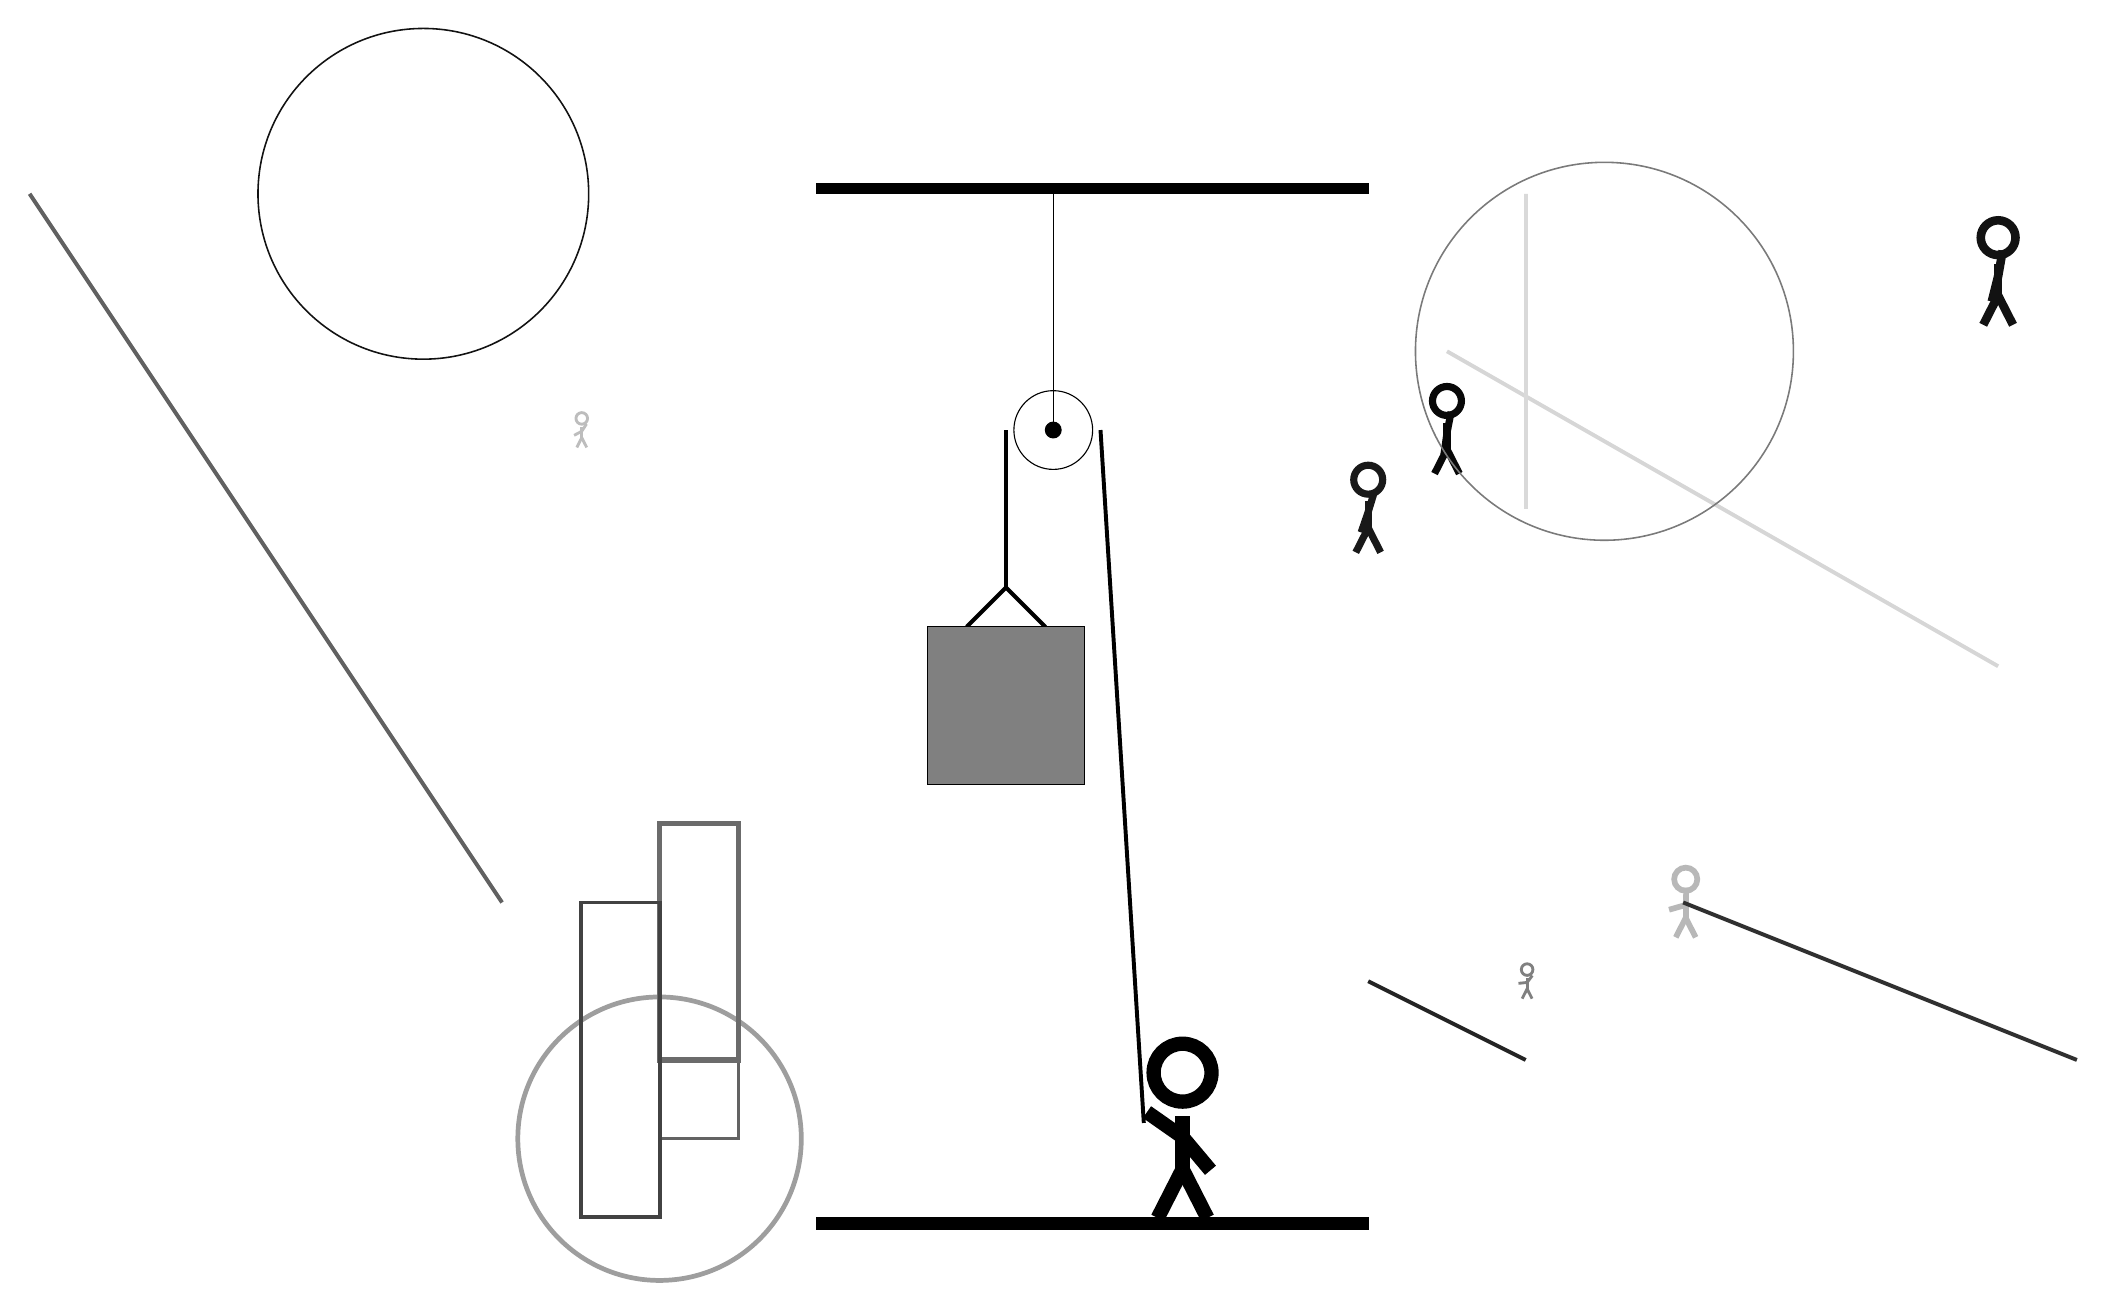
\begin{tikzpicture}
		%%%%% START %%%%%
		
		\draw[fill=black] (-2, 10) rectangle (5, 10.125);
		
		\draw (1, 7) circle (0.5);
		\draw[fill=black] (1, 7) circle (0.1);
		\draw (1, 10) -- (1, 7);
		
		\draw[line width=0.5mm] (-0.1, 4.5) -- (0.4, 5.0) -- (0.9, 4.5);
		\draw[fill=black!50] (-0.6, 4.5) rectangle (1.4, 2.5);
		
		\draw[line width=0.5mm] (0.4, 7) -- (0.4, 5.0);
		\centerarc[line width=0.5mm](1, 7)(0:180:0.6);
		\draw[line width=0.5mm](1.6, 7) -- (2.15, -1.8);
		
		\node at (2.6, -1.9) {\Strichmaxerl[10][-35][-50]};
		
		\node[line width=0.6mm, color=black!26] at (-5, 7) {\Strichmaxerl[2][28][57]};
		
		\draw[line width=0.5mm, color=black!16](6, 8) -- (13, 4);
		\draw[line width=0.5mm, color=black!86](7, -1) -- (5, 0);
		\draw[line width=0.5mm, color=black!15] (7, 10) rectangle (7, 6);
		\node[line width=0.5mm, color=black!90] at (5, 6) {\Strichmaxerl[5][71][73]};
		\node[line width=0.3mm, color=black!28] at (9, 1) {\Strichmaxerl[4][16][88]};
		\node[line width=0.3mm, color=black!97] at (6, 7) {\Strichmaxerl[5][82][79]};
		
		\node[line width=0.5mm, color=black!50] at (7, 0) {\Strichmaxerl[2][6][53]};
		\draw[line width=0.5mm, color=black!81](9, 1) -- (14, -1);
		\draw[line width=0.4mm, color=black!61] (-4, 2) rectangle (-3, -2);
		
		\draw [line width=0.2mm, color=black!52](8, 8) circle (2.4);
		\draw [line width=0.6mm, color=black!38](-4, -2) circle (1.8);
		\draw[line width=0.7mm, color=black!58] (-3, -1) rectangle (-4, 2);
		
		\node[line width=0.5mm, color=black!93] at (13, 9) {\Strichmaxerl[6][76][80]};
		\draw[line width=0.5mm, color=black!74] (-4, -3) rectangle (-5, 1);
		\draw [line width=0.2mm, color=black!93](-7, 10) circle (2.1);
		
		\draw[line width=0.5mm, color=black!62](-6, 1) -- (-12, 10);
		
		\draw[fill=black] (-2, -3) rectangle (5, -3.15);
		
		%%%%% END %%%%%
	\end{tikzpicture}
\end{document}